\section{Data migration categorizes and risks}
	\label{sec:risks}

The perspective of a data modification is always accompanied by a risk. The risk could be a data loss, a data corruption, a technical failure, a change that brings integrity errors, a change that makes the application no more compatible with the data schema, a missing change and so on. We see they are a lot of different risks. In addition of the risk, the complexity is another factor to consider in a migration. The complexity define the difficulty to write some scripts and the impact they could have. It is quite difficult to be absolute with this axis. In general, the complexity could greatly vary depending on the query types but also from the query purposes.

One another aspect to consider is the technologies used by the application to retrieve and manipulate the data. Depending of these technologies, some modifications have a lower impact or no impact than others. For example, adding a column to a table with no constraint (allows null values, duplicates and so on) will be negligible. The application can use the schema with this additional column without any influence but any insert will produce a null field in the row. This is definitively not a good practice.

We must to be careful about the database server used because some of them does not support transactions for all the query types. For example, MySQL\cite{mysql} server does not support transactions for DDL\cite{ddl}. All schema modifications could not be rolled back automatically by the database server. This could have a real impact on migrations. Having queries with transaction supports mixed with no-transaction queries does not make any sense. If it fails during the migration, we have to rollback all the queries or to find a way to retrieve the state of the error and start again from there. This is not a trivial task.

Our experience allows us to categorize the migration by type of changes and complexity and risk. On the figure \ref{risksTable}, you can see our appreciation of the different migration types.

\begin{figure}[h]
        \centering
        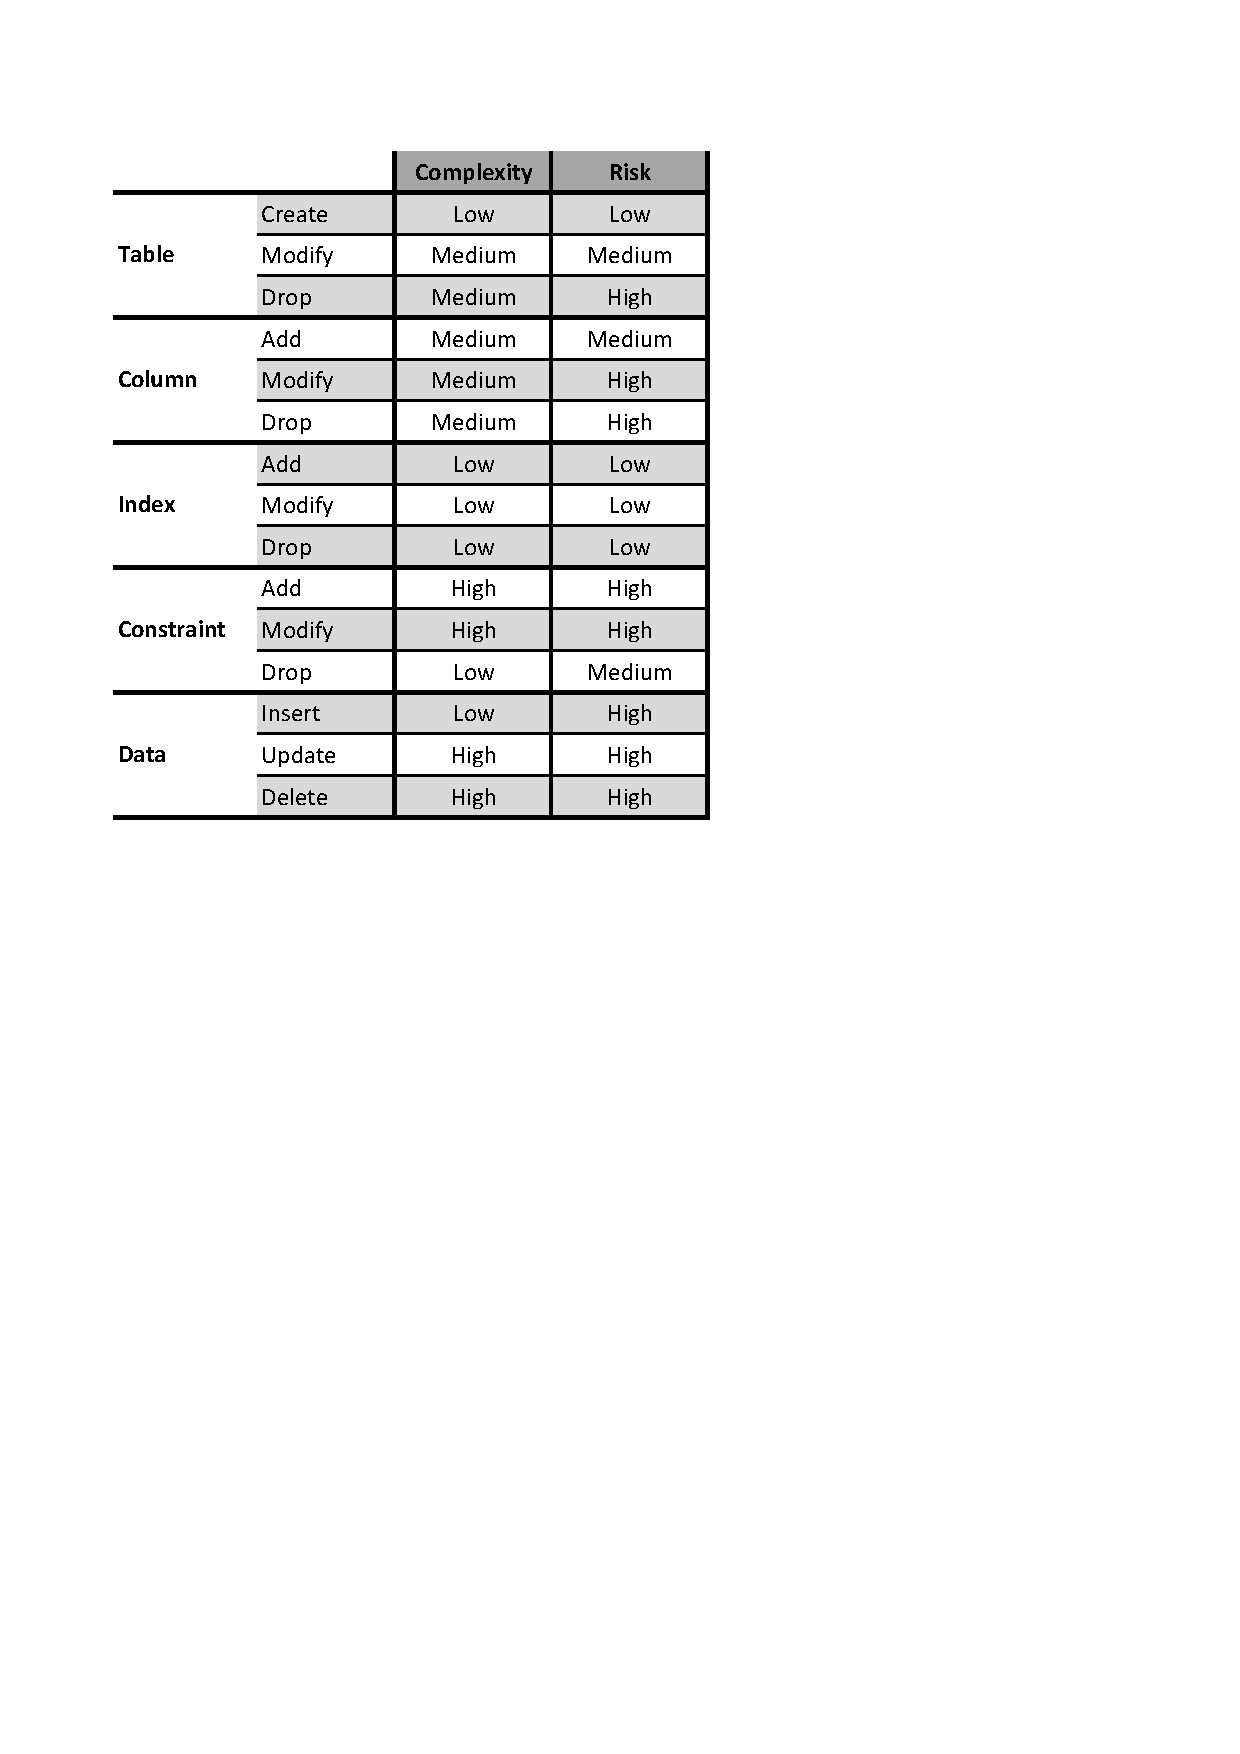
\includegraphics[scale=0.7]{images/risks.pdf}
        \caption{Risks table}
        \label{risksTable}
\end{figure}

\subsection{Table migration}

\subsubsection{Create a table\\}

Create a new table is not a big risk for both axis because the table is there to add a new feature. But you have to keep in mind that adding a table could cause some side effects. In fact, when you add a table, you need probably to populate it with data corresponding to the data you already have in your database. This part could be really tricky because you need to create data based on what you have. This part could be risky or not, it really depends on what is the purpose of your table. There is no absolute rules to define if the addition of a table implies a low or high risk on your business.

\subsubsection{Modify a table\\}

In this case, a modification means to rename the table. The complexity is medium because the command to change the name is quite easy to write, to test and validate. The risk is limited because you only change the name of your table and you would not alter the table content. So you do not risk to loose or corrupt data. If the change is not managed correctly, you risk to have an interruption of service during the time that your application is not mapped to the correct table name.

\subsubsection{Drop a table\\}

Dropping a table is quite easy from complexity point of view. The command is easy to write and test like the renaming command but from the risk point of view it is clearly a major risk. You need to have the insurance that dropping a table is ok and will not produce a non-wanted data loss. You maybe have to think about an archiving procedure before dropping the table and erasing all its content.

\subsection{Column migration}

\subsubsection{Add a column\\}

As we have already briefly discussed, adding a column to a table is not necessary risky. In general, this is not but sometimes, the nature of the column will imply a risk due to the fact that you need to fill in the column with data. In this situation, you can encounter two cases. The first is that the data can easily deduct or filled with default value, the second one is more complicated because you need to calculate the data or to fill the empty field with data based on a the context of the data already present in the database. The second case is more risky and complex than the first one.

It is difficult to choose a risk level or complexity level for this kind of migration because it really depends on the data that the column represent. It could be a low risk as it could be a high risk. Filling the column could imply a more complex procedure if the data to fill are calculate or deducted from the data context.

\subsubsection{Modify a column\\}

Technically, modifying a column is not complex. There are several kind of column migration. You could have to rename, change data type, modify the encoding. Renaming a column is probably the lowest complexity you could have in a migration while a data type change is a bigger complexity. When you change a column type, you risk to truncate your data, loss precision when float are stored and other strange behaviors that will corrupt your data. Changing the encoding has the same kind of risk as the type change.

\subsubsection{Drop a column\\}

Dropping a column is specially risky for the due to the fact you can loose data if you manage the modification incorrectly. You have to take care about the impact of the database. For the complexity point of view, removing a column is not a problem if in the application there is no more reference to this column. Your application can live with a small overload of data implied by a column not dropped that normally must. The complexity could be higher when the column is a foreign key to another table. This kind of modification are always more complex to manage.

\subsection{Index migration}

The index manipulation is probably the lowest risk in database migration. The queries are quite simple and do not imply data directly. We mean that the data stored in your tables remains the same when you manipulate indexes. One risk is on the performance point of view when you add a non-relevant index or when you drop a crucial index that improve your performance.

One thing that could happen is that a migration of your data required an index that is not present. An index missing could implies a very big problem in terms of performance. Some migration that requires few minutes to be executed, could in case of index missing take tens of minutes to be executed with a downtime of your application or service for this time. When a migration is required, taking a look of the indexes must be really useful to avoid lack of performance.

\subsection{Constraint migration}

The constraint migration is a category that implies more subsequent migrations. In general, you need to prepare your database when you add a constraint, you have to correct your database when you remove or update a constraint.

\subsubsection{Add a constraint\\}

Adding a constraint is not easy. It really depends on your data you already have in your database. For example, if you add a constraint that check if a value is unique across a table, you need to check before adding the constraint if there is no duplicates in your data otherwise you will not be able to add the constraint. In this case, you have to decide what to do with duplicates. This is the part that is not easy. Depending the situation, you will not be able to manage easily the duplicates.

\subsubsection{Modify a constraint\\}

As the same as adding a constraint, the modification of one constraint implies the same kind of troubles. You will have to analyze carefully the data you manipulate through your constraint modification to know what to do with them. It is really dependent of the context.

\subsubsection{Drop a constraint\\}

We think that dropping a constraint is not a big complexity because, in general, this relax the constraints imposed to the data. On the other side, risk is quite low, removing a constraint could cause some insidious long terms errors. You have to clarify why a constraint must be removed. You have to guaranty that your application will ensure some correctness of your data. For performance aspects, removing the constrain will be useful but will imply a major risk on your data and especially if your application is not robust or when you have more than one application against the same database. Some data corruption could happens and will not be seen for a while.

\subsection{Data migration}

On all migration category, the data manipulation is the most risky and complex. You can easily corrupt the data in your database without perceiving any problems before a while. Some corruption will appear only after a certain time when your application run into some border case for example. In this case, the correction of the data could be really tricky. The complexity comes from the data themselves. Depending on the data, your migration could be easy or really tricky. You need to know exactly your data to update them.

\subsubsection{Insert data\\}

Inserting data is quite easy for complexity aspects but could be risky. You can easily imagine a case that when you insert new data, you expose them to the wrong public if your system offers a security filtering of your data. You can also exchange text column in a request without an error at the time of your migration but the final customers could see strange texts or strange behaviors that are not easy to detect.

\subsubsection{Update data\\}

When an update is run in a database, if the query is wellformed but semantically erroneous, you risk to update more data than you expect. This is a major risk. Imagine that you have a table with a field name that is unique and you have no constraint on the table to enforce that. Running a query that update this name without specifying a restricting clause to only the record you want to update could cause an update on all your records. If the application relies on name are unique, the application will not be able to handle the data correctly if the records' name are all the same. This is a school case, so one more concrete example. Imagine you have a table to manage Internationalization with a name and a string corresponding to the name. If an update is run without specifying the specific record where to update the string, all the records will see their value changed. In this case, all the translations will have the same wording that is really bad for the final user.

\subsubsection{Delete data\\}

The high risk in deleting data is principally the loss of data that is really critical for a company. In regards of the data, the application could be totally broken after a data deletion. The complexity could be quite high due to the references to other tables. Especially when you have circular references (not a best practice at all).